% PGease — Investor / demo presentation
% Compile with:  pdflatex presentation.tex   (run twice for positioning)
% Requires a standard TeX Live / MiKTeX install with beamer, tikz, booktabs.

\documentclass[aspectratio=169]{beamer}
\usetheme{Madrid}
\usecolortheme{default}

\usepackage[T1]{fontenc}
\usepackage{tikz}
\usetikzlibrary{arrows.meta, positioning}
\usepackage{booktabs}

% ---- PGease brand colours ----
\definecolor{indigo}{RGB}{99,102,241}
\definecolor{violet}{RGB}{139,92,246}
\definecolor{fuchsia}{RGB}{217,70,239}
\definecolor{emerald}{RGB}{16,185,129}
\definecolor{amber}{RGB}{245,158,11}
\definecolor{rose}{RGB}{244,63,94}

\setbeamercolor{structure}{fg=indigo}
\setbeamercolor{frametitle}{bg=indigo, fg=white}
\setbeamercolor{title}{fg=indigo}
\setbeamercolor{itemize item}{fg=violet}
\setbeamercolor{itemize subitem}{fg=indigo}
\setbeamerfont{frametitle}{size=\Large, series=\bfseries}

\title{PGease — one platform, two faces}
\subtitle{Find a verified PG near your work. Or fill yours faster.}
\author{Hyderabad-first · built to go national}
\date{September 2026}

\titlegraphic{%

\begin{tikzpicture}
  \fill[indigo] (0,0) rectangle (1.4,1.4);
  \fill[violet] (0.7,0.7) rectangle (1.4,1.4);
  \draw[white, thick, line cap=round, line join=round]
    (-0.35,0.6) -- (0.35,1.15) -- (1.05,1.15) -- (1.05,0.6) -- cycle;
  \fill[white] (-0.05,0.6) rectangle (0.35,0.95);
\end{tikzpicture}%
}

\begin{document}

% ============================================================ TITLE
\begin{frame}
  \titlepage
\end{frame}

% ============================================================ BIG IDEA
\begin{frame}{The big idea}
  \begin{center}
    \Large
    Hyderabad's PG network is an \textbf{unbuilt hotel network}\\ that already exists — \\
    and nobody can see it.
  \end{center}
  \vspace{0.4cm}
  \begin{block}{}
    One dataset, two faces: \textbf{tenants} search verified PGs by commute and budget;
    \textbf{owners} run the whole business and get the tenants.
  \end{block}
\end{frame}

% ============================================================ PROBLEM: TENANTS
\begin{frame}{The problem — for tenants}
  \begin{itemize}
    \item \textbf{No live availability.} Listings tell you a PG \emph{exists}, not whether a bed is free tonight.
    \item \textbf{Commute is unknown.} Proximity is how rent is priced, but no one shows travel time to \emph{your} office or college.
    \item \textbf{Trust is broken.} Fake photos, fake reviews, deposit disputes, curfews.
    \item \textbf{Budget guessing.} No way to filter by \emph{your} number across rooms and localities.
  \end{itemize}
  \vspace{0.2cm}
  \begin{alertblock}{Quantified}
    446 airport-touting cases a year; travel agents admit ``hardly anyone to give information when someone asks.''
  \end{alertblock}
\end{frame}

% ============================================================ PROBLEM: OWNERS
\begin{frame}{The problem — for owners}
  \begin{itemize}
    \item \textbf{Fragmented and informal.} Runs on registers and WhatsApp; cash and UPI mixed.
    \item \textbf{Compliance is now mandatory.} Jul 2026 audit of 447 women's hostels:
      \textbf{44\%} valid licence, \textbf{0\%} fire-exit plan, \textbf{62\%} scored below 40/100.
    \item \textbf{GST confusion.} Owners charge cash and threaten a 12\% surcharge they often \emph{don't owe}.
    \item \textbf{Vacancy is their \#1 silent cost.} Empty bed = Rs.\ 0/month, and no demand channel.
  \end{itemize}
\end{frame}

% ============================================================ OPPORTUNITY
\begin{frame}{The opportunity is enormous}
  \begin{columns}
    \column{0.46\textwidth}
      \begin{itemize}
        \item \textbf{6.6M} beds demanded vs \textbf{0.3M} organised — \textbf{$<$5\%} penetration
        \item Market: \textbf{Rs.\ 40 bn} (2025) $\rightarrow$ \textbf{Rs.\ 206 bn} (2030)
        \item \textbf{447} hostels in one Hyderabad police zone alone
        \item Regulation (Project Safe Stay) is \emph{forcing} digitisation now
      \end{itemize}
    \column{0.54\textwidth}
      \begin{center}
        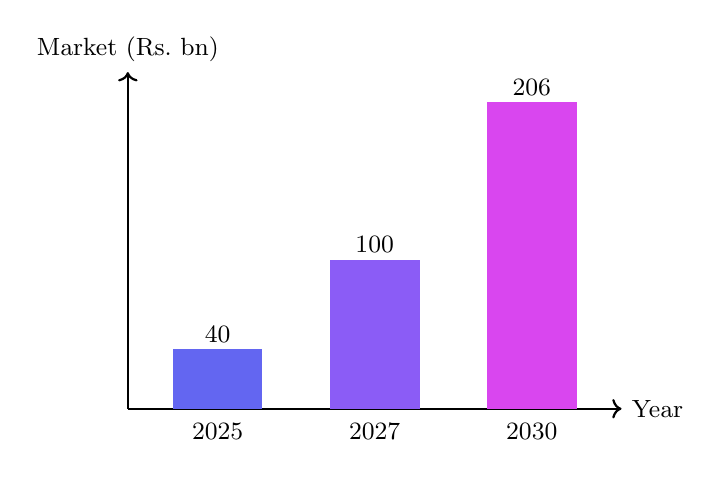
\begin{tikzpicture}[scale=0.95]
          \draw[->, thick] (0,0) -- (0,4.5) node[above, font=\small]{Market (Rs.\ bn)};
          \draw[->, thick] (0,0) -- (6.6,0) node[right, font=\small]{Year};
          \fill[indigo] (0.6,0) rectangle (1.8,{40/206*4.1});
          \node[font=\small] at (1.2,{40/206*4.1+0.2}) {40};
          \fill[violet] (2.7,0) rectangle (3.9,{100/206*4.1});
          \node[font=\small] at (3.3,{100/206*4.1+0.2}) {100};
          \fill[fuchsia] (4.8,0) rectangle (6.0,4.1);
          \node[font=\small] at (5.4,4.3) {206};
          \node[font=\small] at (1.2,-0.3) {2025};
          \node[font=\small] at (3.3,-0.3) {2027};
          \node[font=\small] at (5.4,-0.3) {2030};
        \end{tikzpicture}
        \\[0.2cm]
        {\small Source: Colliers India, 2025}
      \end{center}
  \end{columns}
\end{frame}

% ============================================================ SOLUTION
\begin{frame}{The solution — two faces, one dataset}
  \begin{center}
    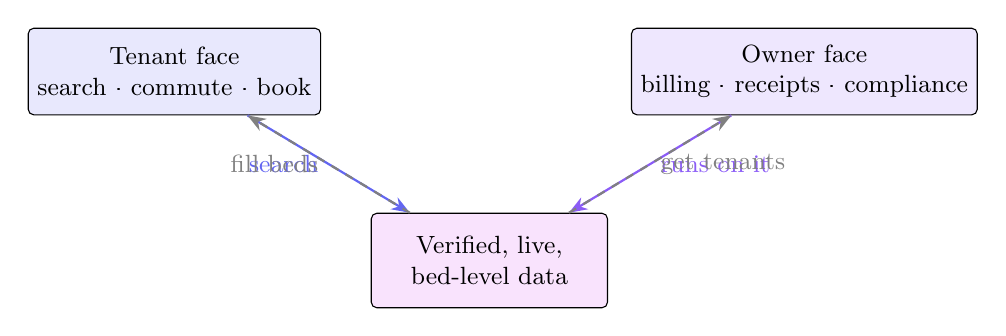
\begin{tikzpicture}[
        box/.style={draw, rounded corners=2pt, minimum width=3.0cm, minimum height=1.1cm,
                    align=center, font=\small},
      ]
      \node[box, fill=indigo!15] (tenant) at (0,0) {Tenant face\\ search · commute · book};
      \node[box, fill=violet!15] (owner) at (8,0) {Owner face\\ billing · receipts · compliance};
      \node[box, fill=fuchsia!15, minimum height=1.2cm] (data) at (4,-2.4) {Verified, live,\\ bed-level data};
      \draw[-{Stealth}, thick, indigo] (tenant) -- (data) node[midway, left, font=\small]{search};
      \draw[-{Stealth}, thick, violet] (owner) -- (data) node[midway, right, font=\small]{runs on it};
      \draw[-{Stealth}, thick, dashed, gray] (data) -- (tenant) node[midway, left, font=\small]{fill beds};
      \draw[-{Stealth}, thick, dashed, gray] (data) -- (owner) node[midway, right, font=\small]{get tenants};
    \end{tikzpicture}
  \end{center}
  \vspace{0.2cm}
  \begin{block}{Why it wins}
    Not a listings site, not an operator — the \textbf{operating layer} that produces the
    live, verified data nobody else has.
  \end{block}
\end{frame}

% ============================================================ FLYWHEEL
\begin{frame}{The flywheel}
  \begin{center}
    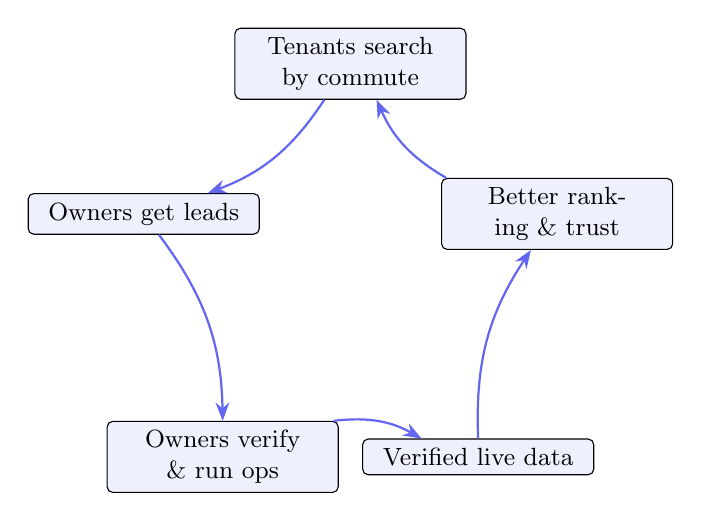
\begin{tikzpicture}[scale=0.92]
      \foreach \a/\t in {
          90/Tenants search by commute,
          162/Owners get leads,
          234/Owners verify \& run ops,
          306/Verified live data,
          18/Better ranking \& trust} {
        \node[draw, rounded corners=2pt, fill=indigo!10, text width=2.7cm, align=center, font=\small]
          (n\a) at (\a:3.0) {\t};
      }
      \draw[-{Stealth}, thick, indigo] (n90) to[bend left=18] (n162);
      \draw[-{Stealth}, thick, indigo] (n162) to[bend left=18] (n234);
      \draw[-{Stealth}, thick, indigo] (n234) to[bend left=18] (n306);
      \draw[-{Stealth}, thick, indigo] (n306) to[bend left=18] (n18);
      \draw[-{Stealth}, thick, indigo] (n18) to[bend left=18] (n90);
    \end{tikzpicture}
  \end{center}
  \begin{center}
    {\small The same verification that protects tenants is what ranks owners higher.}
  \end{center}
\end{frame}

% ============================================================ TECH STACK
\begin{frame}{Tech stack — what we built (front-end prototype)}
  \begin{columns}
    \column{0.52\textwidth}
      \begin{table}
        \small
        \begin{tabular}{ll}
          \toprule
          Layer & Choice \\
          \midrule
          Frontend & React 19 + TypeScript \\
          Build & Vite 7 \\
          UI & Tailwind CSS v4 + lucide \\
          Routing & React Router 7 \\
          State & Zustand (persisted) \\
          Maps & Leaflet + OpenStreetMap \\
          Domain & GST engine, commute logic \\
          \bottomrule
        \end{tabular}
      \end{table}
    \column{0.48\textwidth}
      \begin{itemize}
        \item Zero backend — runs on localStorage, works offline
        \item Class-based dark mode, PWA-ready
        \item Hash routing — hosts anywhere
      \end{itemize}
  \end{columns}
\end{frame}

\begin{frame}{Planned production architecture}
  \begin{center}
    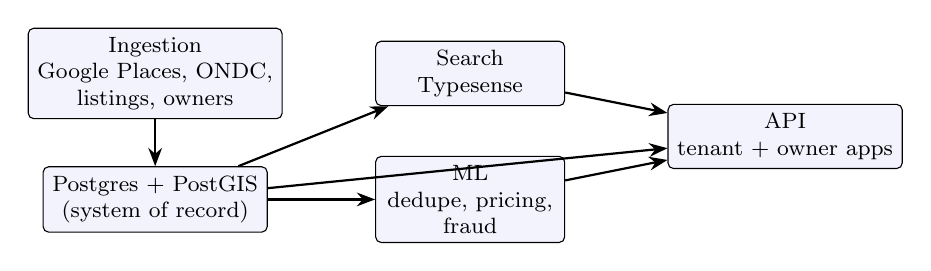
\begin{tikzpicture}[
        box/.style={draw, rounded corners=2pt, fill=indigo!8, align=center,
                    minimum width=2.4cm, minimum height=0.8cm, font=\footnotesize},
        lbl/.style={font=\footnotesize, text=indigo}
      ]
      \node[box] (ing) at (0,2.2) {Ingestion\\ Google Places, ONDC,\\ listings, owners};
      \node[box] (pg) at (0,0.6) {Postgres + PostGIS\\ (system of record)};
      \node[box] (srch) at (4,2.2) {Search\\ Typesense};
      \node[box] (ml) at (4,0.6) {ML\\ dedupe, pricing,\\ fraud};
      \node[box] (api) at (8,1.4) {API\\ tenant + owner apps};
      \draw[-{Stealth}, thick] (ing) -- (pg);
      \draw[-{Stealth}, thick] (pg) -- (srch);
      \draw[-{Stealth}, thick] (pg) -- (ml);
      \draw[-{Stealth}, thick] (srch) -- (api);
      \draw[-{Stealth}, thick] (ml) -- (api);
      \draw[-{Stealth}, thick] (pg) -- (api);
    \end{tikzpicture}
  \end{center}
\end{frame}

% ============================================================ TENANT
\begin{frame}{Tenant experience}
  \begin{itemize}
    \item Search by \textbf{locality}, \textbf{commute} and \textbf{your own budget}
    \item Live map with price pins (desktop + mobile)
    \item Per-listing: verified badge, compliance status, reviews, pricing
    \item \textbf{Request a visit} $\rightarrow$ lands in the owner's inbox
  \end{itemize}
  \vspace{0.25cm}
  \begin{center}
    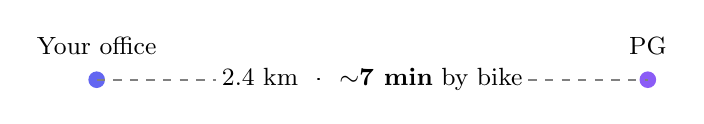
\begin{tikzpicture}
      \fill[indigo] (0,0) circle (3pt);
      \node[font=\small, above] at (0,0.2) {Your office};
      \fill[violet] (7,0) circle (3pt);
      \node[font=\small, above] at (7,0.2) {PG};
      \draw[thick, dashed, gray] (0,0) -- (7,0);
      \node[font=\small, fill=white, inner sep=2pt] at (3.5,0) {2.4 km \ · \ \textbf{$\sim$7 min} by bike};
    \end{tikzpicture}
  \end{center}
  \begin{center}
    {\small Commute = straight-line distance + time estimates now; real routing (OSRM / Distance Matrix) later.}
  \end{center}
\end{frame}

% ============================================================ OWNER
\begin{frame}{Owner experience}
  \begin{columns}
    \column{0.5\textwidth}
      \begin{itemize}
        \item Dashboard: occupancy, rent roll, dues
        \item Rooms \& tenants: bed-level inventory
        \item Billing with auto-\textbf{GST}
        \item Electricity, food, compliance vault
        \item \textbf{Leads} inbox
      \end{itemize}
    \column{0.5\textwidth}
      \begin{itemize}
        \item Printable, GST-compliant \textbf{receipts}
        \item Expiry alerts for licence / fire NOC / FSSAI
        \item Verified badge $\Rightarrow$ higher ranking
      \end{itemize}
  \end{columns}
\end{frame}

% ============================================================ GST
\begin{frame}{The GST engine — automatic and correct}
  \begin{center}
    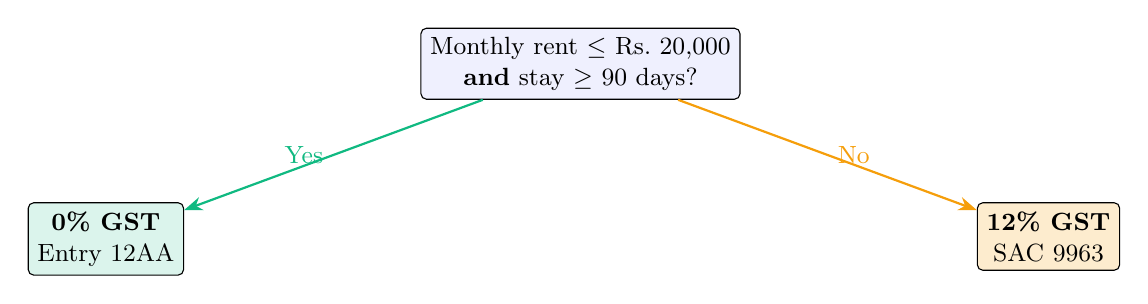
\begin{tikzpicture}[
        node distance=1.3cm and 3.0cm,
        q/.style={draw, rounded corners=2pt, fill=indigo!10, align=center, font=\small},
      ]
      \node[q] (q) {Monthly rent $\le$ Rs.\ 20,000\\ \textbf{and} stay $\ge$ 90 days?};
      \node[q, fill=emerald!15] (yes) [below left=of q] {\textbf{0\% GST}\\ Entry 12AA};
      \node[q, fill=amber!20] (no) [below right=of q] {\textbf{12\% GST}\\ SAC 9963};
      \draw[-{Stealth}, thick, emerald] (q) -- (yes) node[midway, left, font=\small]{Yes};
      \draw[-{Stealth}, thick, amber] (q) -- (no) node[midway, right, font=\small]{No};
    \end{tikzpicture}
  \end{center}
  \begin{itemize}
    \item Every receipt prints the correct declaration
    \item Electricity treated as a pass-through (no GST)
    \item Turns owner tax anxiety into a \textbf{feature}
  \end{itemize}
\end{frame}

% ============================================================ VERIFICATION
\begin{frame}{Fraud prevention — verify before listing}
  \begin{columns}
    \column{0.5\textwidth}
      A 4-step owner onboarding:
      \begin{enumerate}
        \item Owner (name, phone)
        \item Property (address, PIN)
        \item \textbf{Verification} — GSTIN, photos, GPS
        \item Review $\rightarrow$ \emph{verification pending}
      \end{enumerate}
    \column{0.5\textwidth}
      Production plan:
      \begin{itemize}
        \item OTP (Twilio / MSG91)
        \item GSTIN lookup (Razorpay / Cleartax)
        \item GPS $\times$ address cross-check
        \item Admin approve / reject
      \end{itemize}
  \end{columns}
\end{frame}

% ============================================================ HONESTY
\begin{frame}{What is real vs simulated today}
  \begin{table}
    \small
    \begin{tabular}{lll}
      \toprule
      Feature & Prototype & Production \\
      \midrule
      Search, filters, map & \textcolor{emerald}{Real} & Real \\
      Commute (distance/time) & \textcolor{emerald}{Real (estimate)} & Real routing \\
      GST engine & \textcolor{emerald}{Real logic} & + GSTIN lookup \\
      Verification capture & \textcolor{emerald}{Real UI} & + OTP, KYC, admin \\
      Payments / OTP / live availability & \textcolor{amber}{Simulated} & Backend \\
      \bottomrule
    \end{tabular}
  \end{table}
\end{frame}

% ============================================================ ROADMAP
\begin{frame}{Roadmap}
  \begin{enumerate}
    \item \textbf{Now} — Hyderabad depth: backend (Postgres, auth, UPI), convert owners
    \item \textbf{Then} — Hyderabad coverage: Google Places, ONDC, listings + entity resolution
    \item \textbf{Top 10 cities} — Bengaluru, Pune, Mumbai, Delhi-NCR, Chennai, \dots
    \item \textbf{National + ML} — pricing, fraud, recommendations at scale
  \end{enumerate}
  \vspace{0.3cm}
  \begin{block}{}
    The moat is the operating layer that produces \textbf{verified, live, bed-level} data —
    the thing every listing site lacks.
  \end{block}
\end{frame}

% ============================================================ THANK YOU
\begin{frame}
  \begin{center}
    \Huge \textcolor{indigo}{PGease}\\[0.3cm]
    \Large Find a verified PG near your work. Or fill yours faster.\\[0.6cm]
    \small Hyderabad-first · built to go national
  \end{center}
\end{frame}

\end{document}
